\documentclass[11pt, a4paper]{article}
\usepackage{pdfpages}
\usepackage{parallel}
\usepackage[T2A]{fontenc}
\usepackage{ucs}
\usepackage[utf8x]{inputenc}
\usepackage[polish,english,russian]{babel}
\usepackage{hyperref}
\usepackage{rotating}
\usepackage[inner=2cm,top=1.8cm,outer=2cm,bottom=2.3cm,nohead]{geometry}
\usepackage{listings}
\usepackage{graphicx}
\usepackage{wrapfig}
\usepackage{longtable}
\usepackage{indentfirst}
\usepackage{array}
\usepackage{tikzsymbols}
\usepackage{soul}
\usepackage[ruled,vlined]{algorithm2e}
%\counterwithout{figure}{section} 

\usepackage{url}
\makeatletter
\g@addto@macro{\UrlBreaks}{\UrlOrds}
\makeatother

\newcolumntype{P}[1]{>{\raggedright\arraybackslash}p{#1}}
\frenchspacing
\usepackage{fixltx2e} %text sub- and superscripts
\usepackage{icomma} % коскі ў матэматычным рэжыме
\PreloadUnicodePage{4}

\newcommand{\longpage}{\enlargethispage{\baselineskip}}
\newcommand{\shortpage}{\enlargethispage{-\baselineskip}}

\def\switchlang#1{\expandafter\csname switchlang#1\endcsname}
\def\switchlangbe{
\let\saverefname=\refname%
\def\refname{Літаратура}%
\def\figurename{Іл.}%
}
\def\switchlangen{
\let\saverefname=\refname%
\def\refname{References}%
\def\figurename{Fig.}%
}
\def\switchlangru{
\let\saverefname=\refname%
\let\savefigurename=\figurename%
\def\refname{Литература}%
\def\figurename{Рис.}%
}

\hyphenation{admi-ni-stra-tive}
\hyphenation{ex-pe-ri-ence}
\hyphenation{fle-xi-bi-li-ty}
\hyphenation{Py-thon}
\hyphenation{ma-the-ma-ti-cal}
\hyphenation{re-ported}
\hyphenation{imp-le-menta-tions}
\hyphenation{pro-vides}
\hyphenation{en-gi-neering}
\hyphenation{com-pa-ti-bi-li-ty}
\hyphenation{im-pos-sible}
\hyphenation{desk-top}
\hyphenation{elec-tro-nic}
\hyphenation{com-pa-ny}
\hyphenation{de-ve-lop-ment}
\hyphenation{de-ve-loping}
\hyphenation{de-ve-lop}
\hyphenation{da-ta-ba-se}
\hyphenation{plat-forms}
\hyphenation{or-ga-ni-za-tion}
\hyphenation{pro-gramming}
\hyphenation{in-stru-ments}
\hyphenation{Li-nux}
\hyphenation{sour-ce}
\hyphenation{en-vi-ron-ment}
\hyphenation{Te-le-pathy}
\hyphenation{Li-nux-ov-ka}
\hyphenation{Open-BSD}
\hyphenation{Free-BSD}
\hyphenation{men-ti-on-ed}
\hyphenation{app-li-ca-tion}

\def\progref!#1!{\texttt{#1}}
\renewcommand{\arraystretch}{2} %Іначай формулы ў матрыцы зліпаюцца з лініямі
\usepackage{array}

\def\interview #1 (#2), #3, #4, #5\par{

\section[#1, #3, #4]{#1 -- #3, #4}
\def\qname{LVEE}
\def\aname{#1}
\def\q ##1\par{{\noindent \bf \qname: ##1 }\par}
\def\a{{\noindent \bf \aname: } \def\qname{L}\def\aname{#2}}
}

\def\interview* #1 (#2), #3, #4, #5\par{

\section*{#1\\{\small\rm #3, #4. #5}}
\ifx\ParallelWhichBox\undefined%
    \addcontentsline{toc}{section}{#1, #3, #4}%
\else%
\ifnum\ParallelWhichBox=0%
    \addcontentsline{toc}{section}{#1, #3, #4}%
\fi\fi%

\def\qname{LVEE}
\def\aname{#1}
\def\q ##1\par{{\noindent \bf \qname: ##1 }\par}
\def\a{{\noindent \bf \aname: } \def\qname{L}\def\aname{#2}}
}

\newcommand{\interviewfooter}[1]{
\vskip 1em
\noindent \textit{#1}
}


\begin{document}

\title{1987 "--- MicroSpeed FastTRAP trackball}
\date{}
\maketitle

Устройство FastTRAP от MicroSpeed, выпущенное в 1987 году, представляет собой трекбол с тремя кнопками, а также дополнительным колесом, благодаря которому он может выдавать координаты не по двум, а по трем координатным осям  — \textit{x}, \textit{y} и \textit{z} — то есть поддерживает на одну координатную плоскость больше, чем мышь или планшет (рис. \ref{fig:FastTRAPPic}). Дополнительная ось была рассчитана в первую очередь на пользователей САПР твердотельного моделирования, поскольку именно в них одновременное изменение сразу в трёх координатных осях может сократить время, необходимое для вращения объекта или проекции в окне просмотра.

\begin{figure}[h]
   \centering
    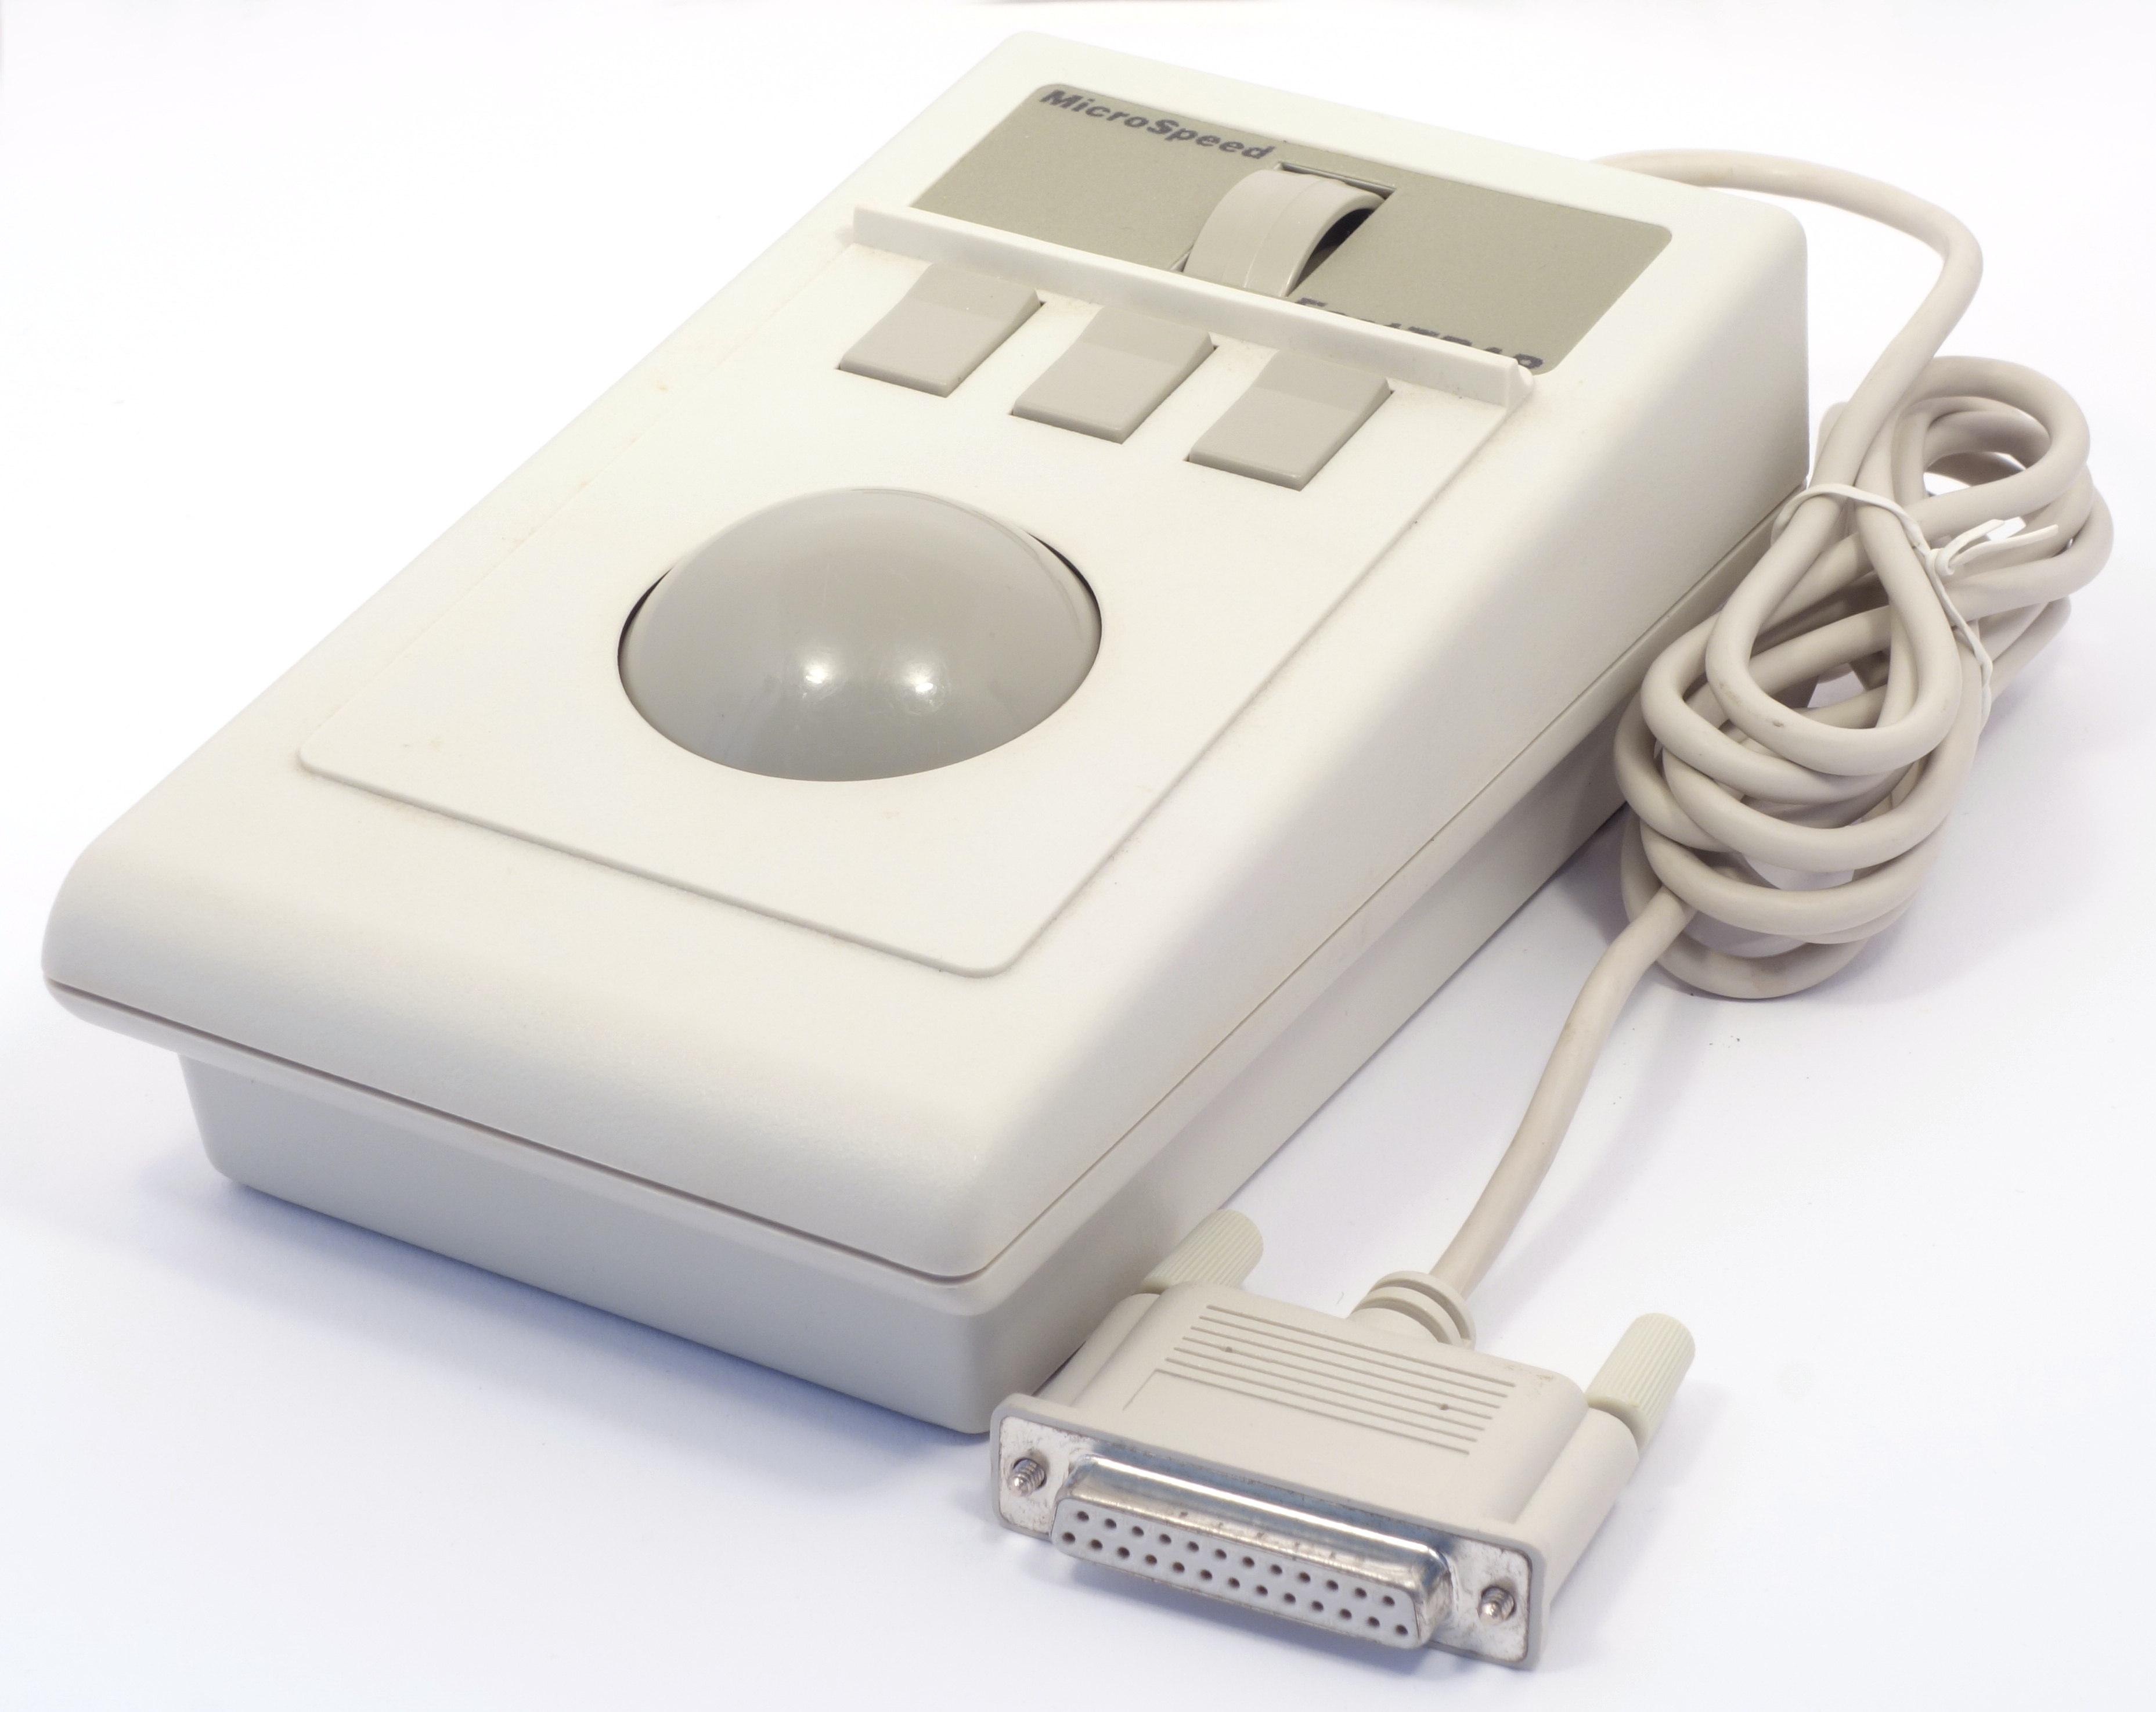
\includegraphics[scale=0.3]{1987_microspeed_fasttrap/pic_15.jpg}
    \caption{MicroSpeed FastTRAP}
    \label{fig:FastTRAPPic}
\end{figure}

Управление по оси \textit{z} осуществляется вращением колеса; однако в момент выпуска этого устройства концепции колеса прокрутки еще не существовало, поэтому программное обеспечение не позволяет использовать его для скроллинга в графических или текстовых программах.

\begin{figure}[h]
    \centering
    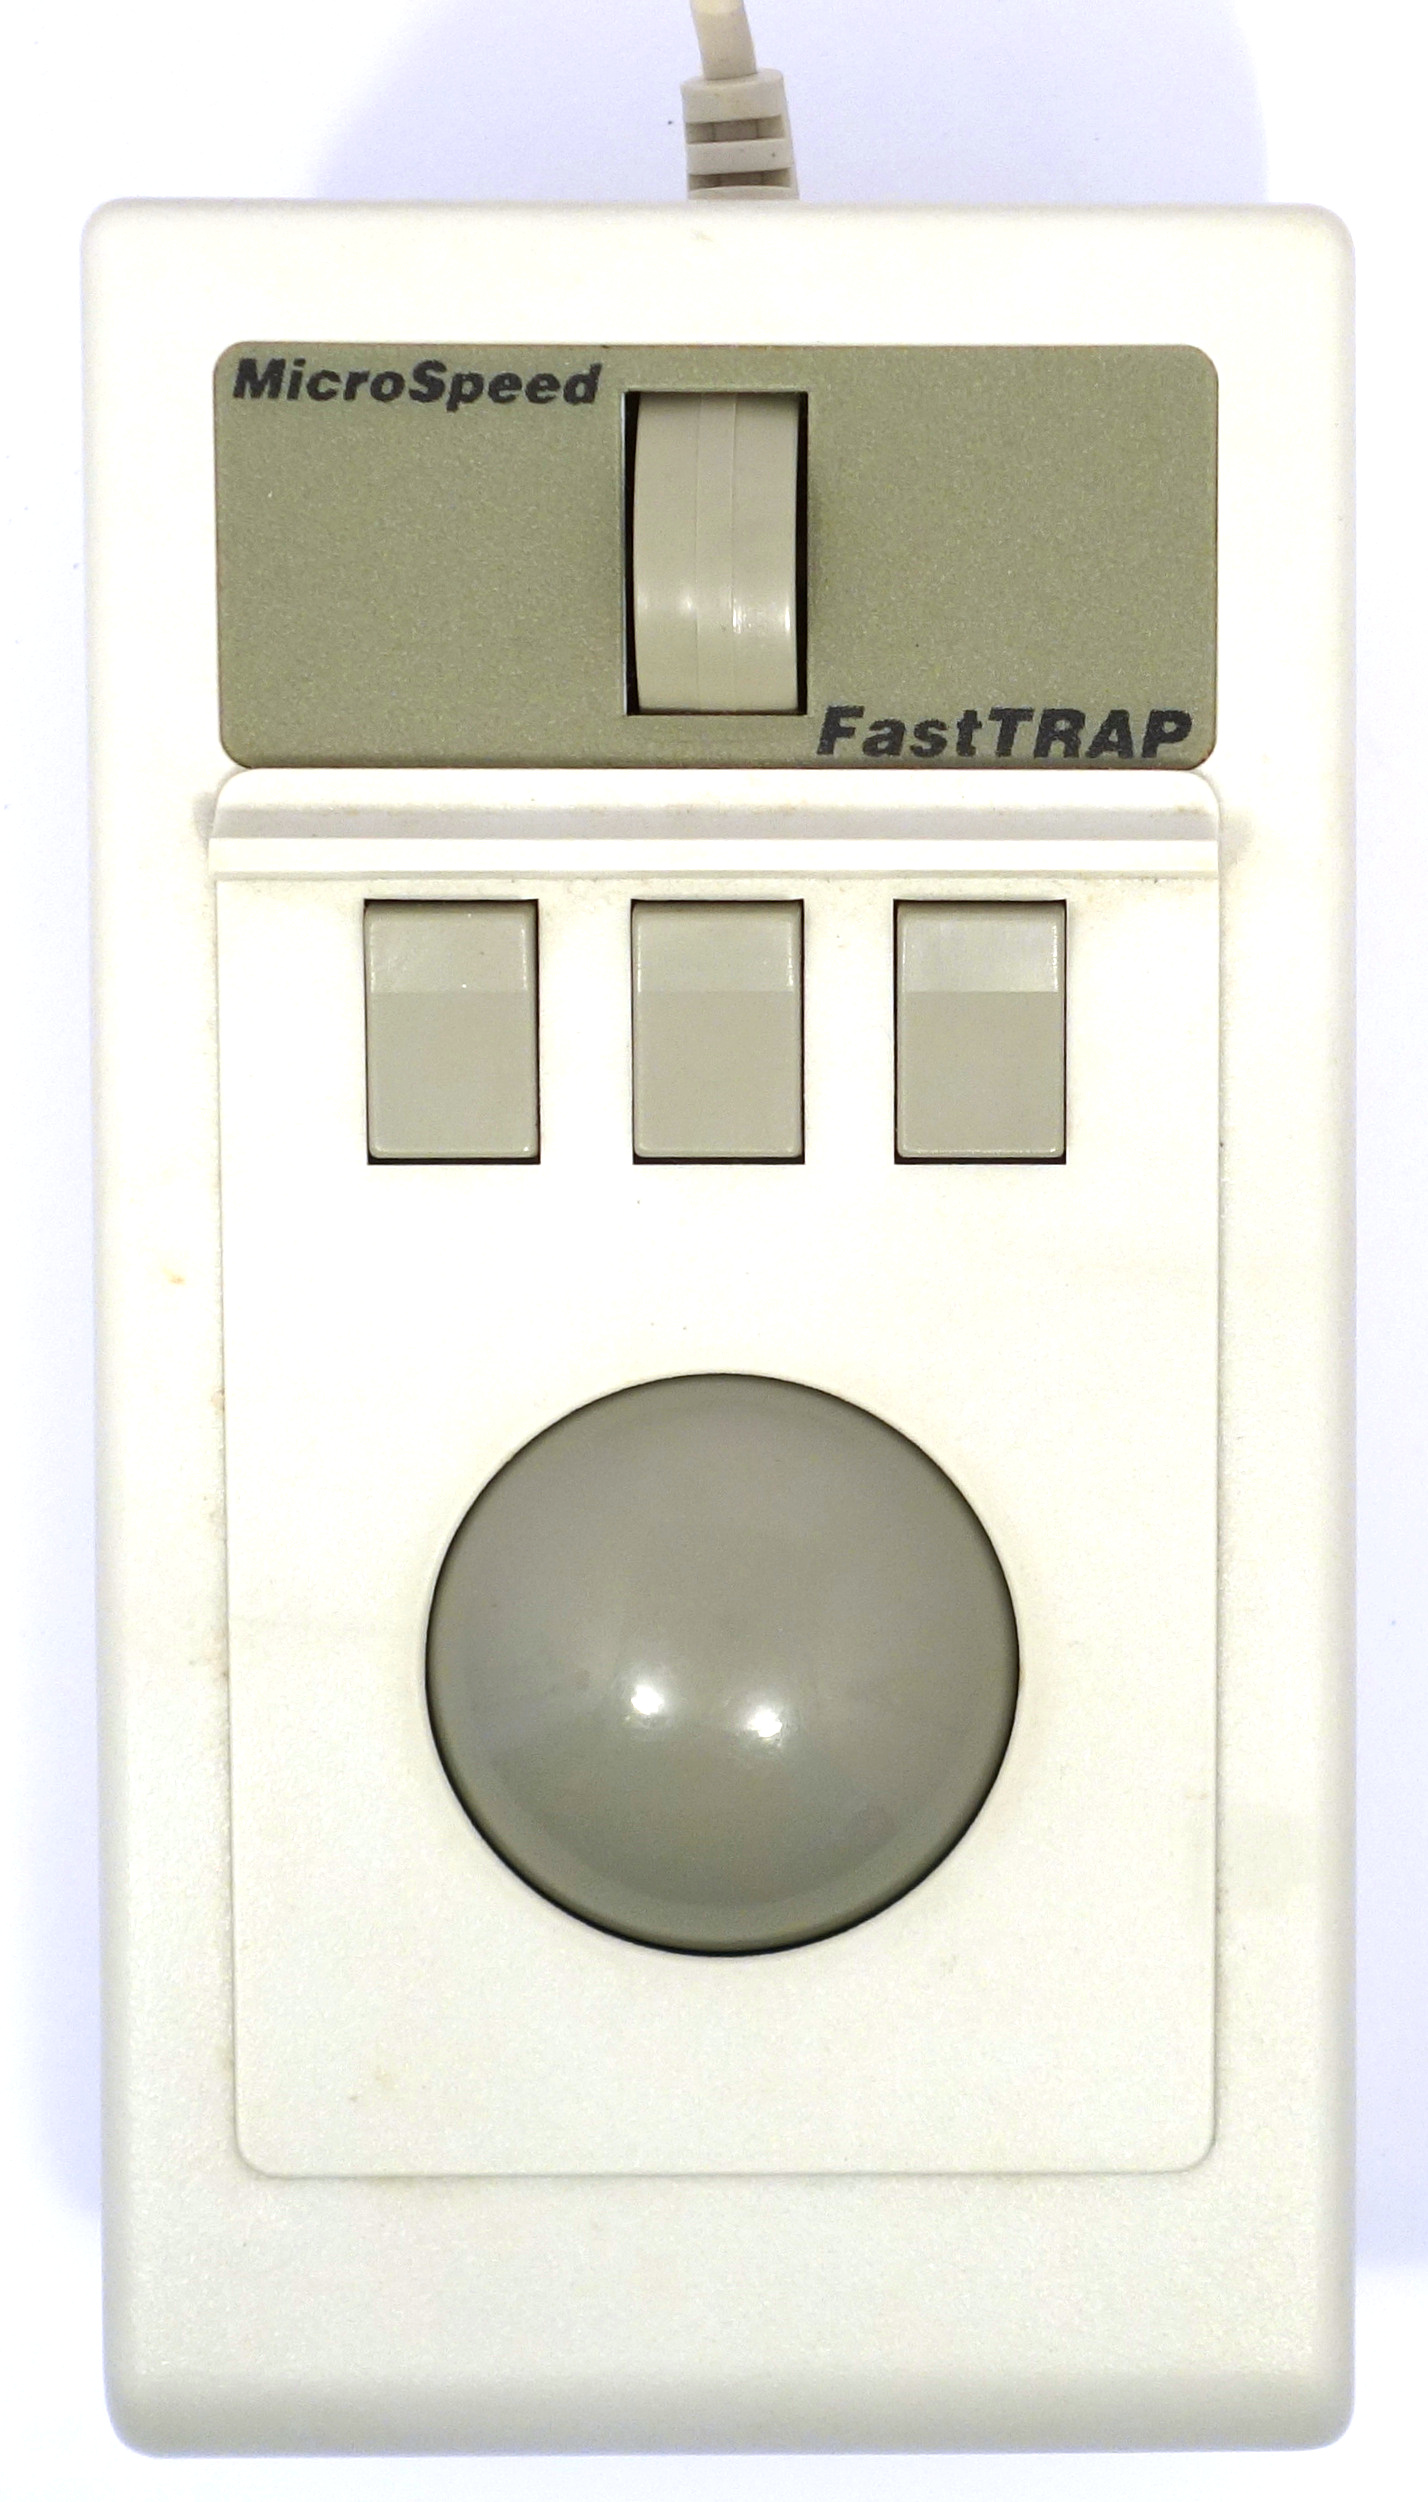
\includegraphics[scale=0.3]{1987_microspeed_fasttrap/top_60.jpg}
    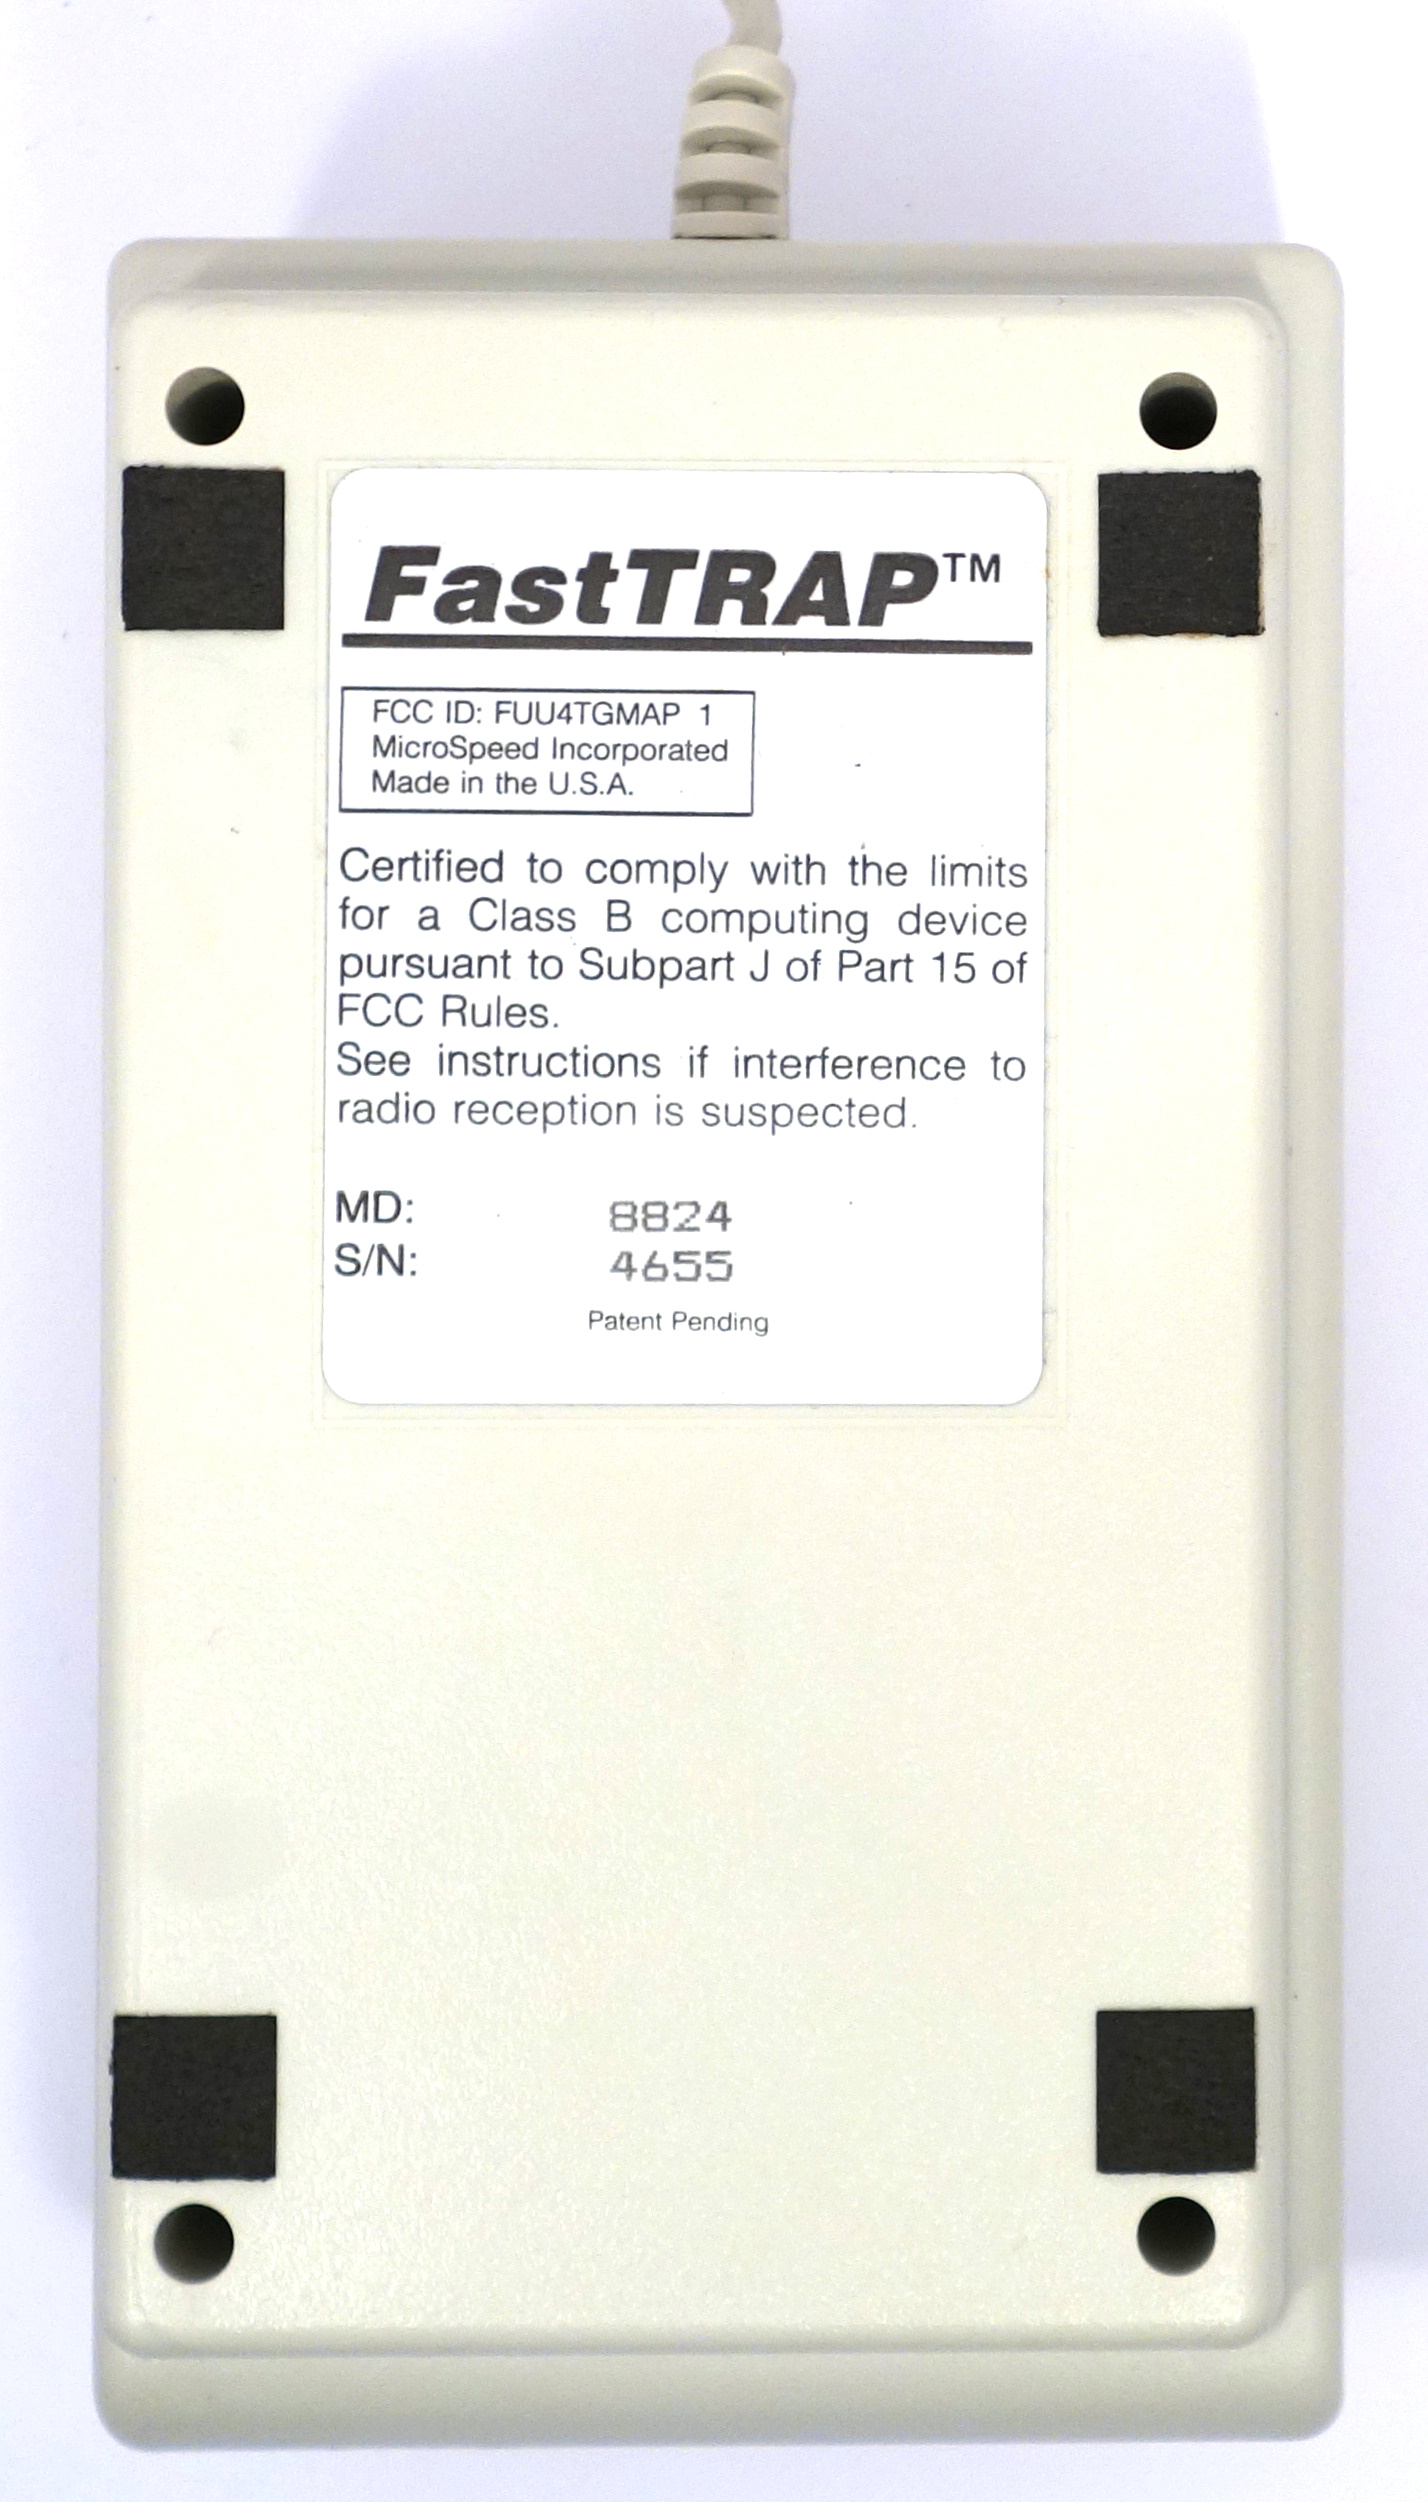
\includegraphics[scale=0.3]{1987_microspeed_fasttrap/bottom_60.jpg}
    \caption{Изображение FastTRAP, вид сверху и снизу}
    \label{fig:FastTRAPTop}
\end{figure}

При подключении к компьютеру FastTRAP использует протокол мыши Microsoft, и может использовать соответствующий стандартный драйвер. Идущий в комплекте специализированный драйвер требуется только для работы с третьей координатой. Также идущая в комплекте программа настройки позволяет запрограммировать функции клавиш, шара и колеса, что позволяет адаптировать устройство под любое программное обеспечение: например выполнять определенные команды DOS \cite{fast}.

\begin{figure}[h]
   \centering
    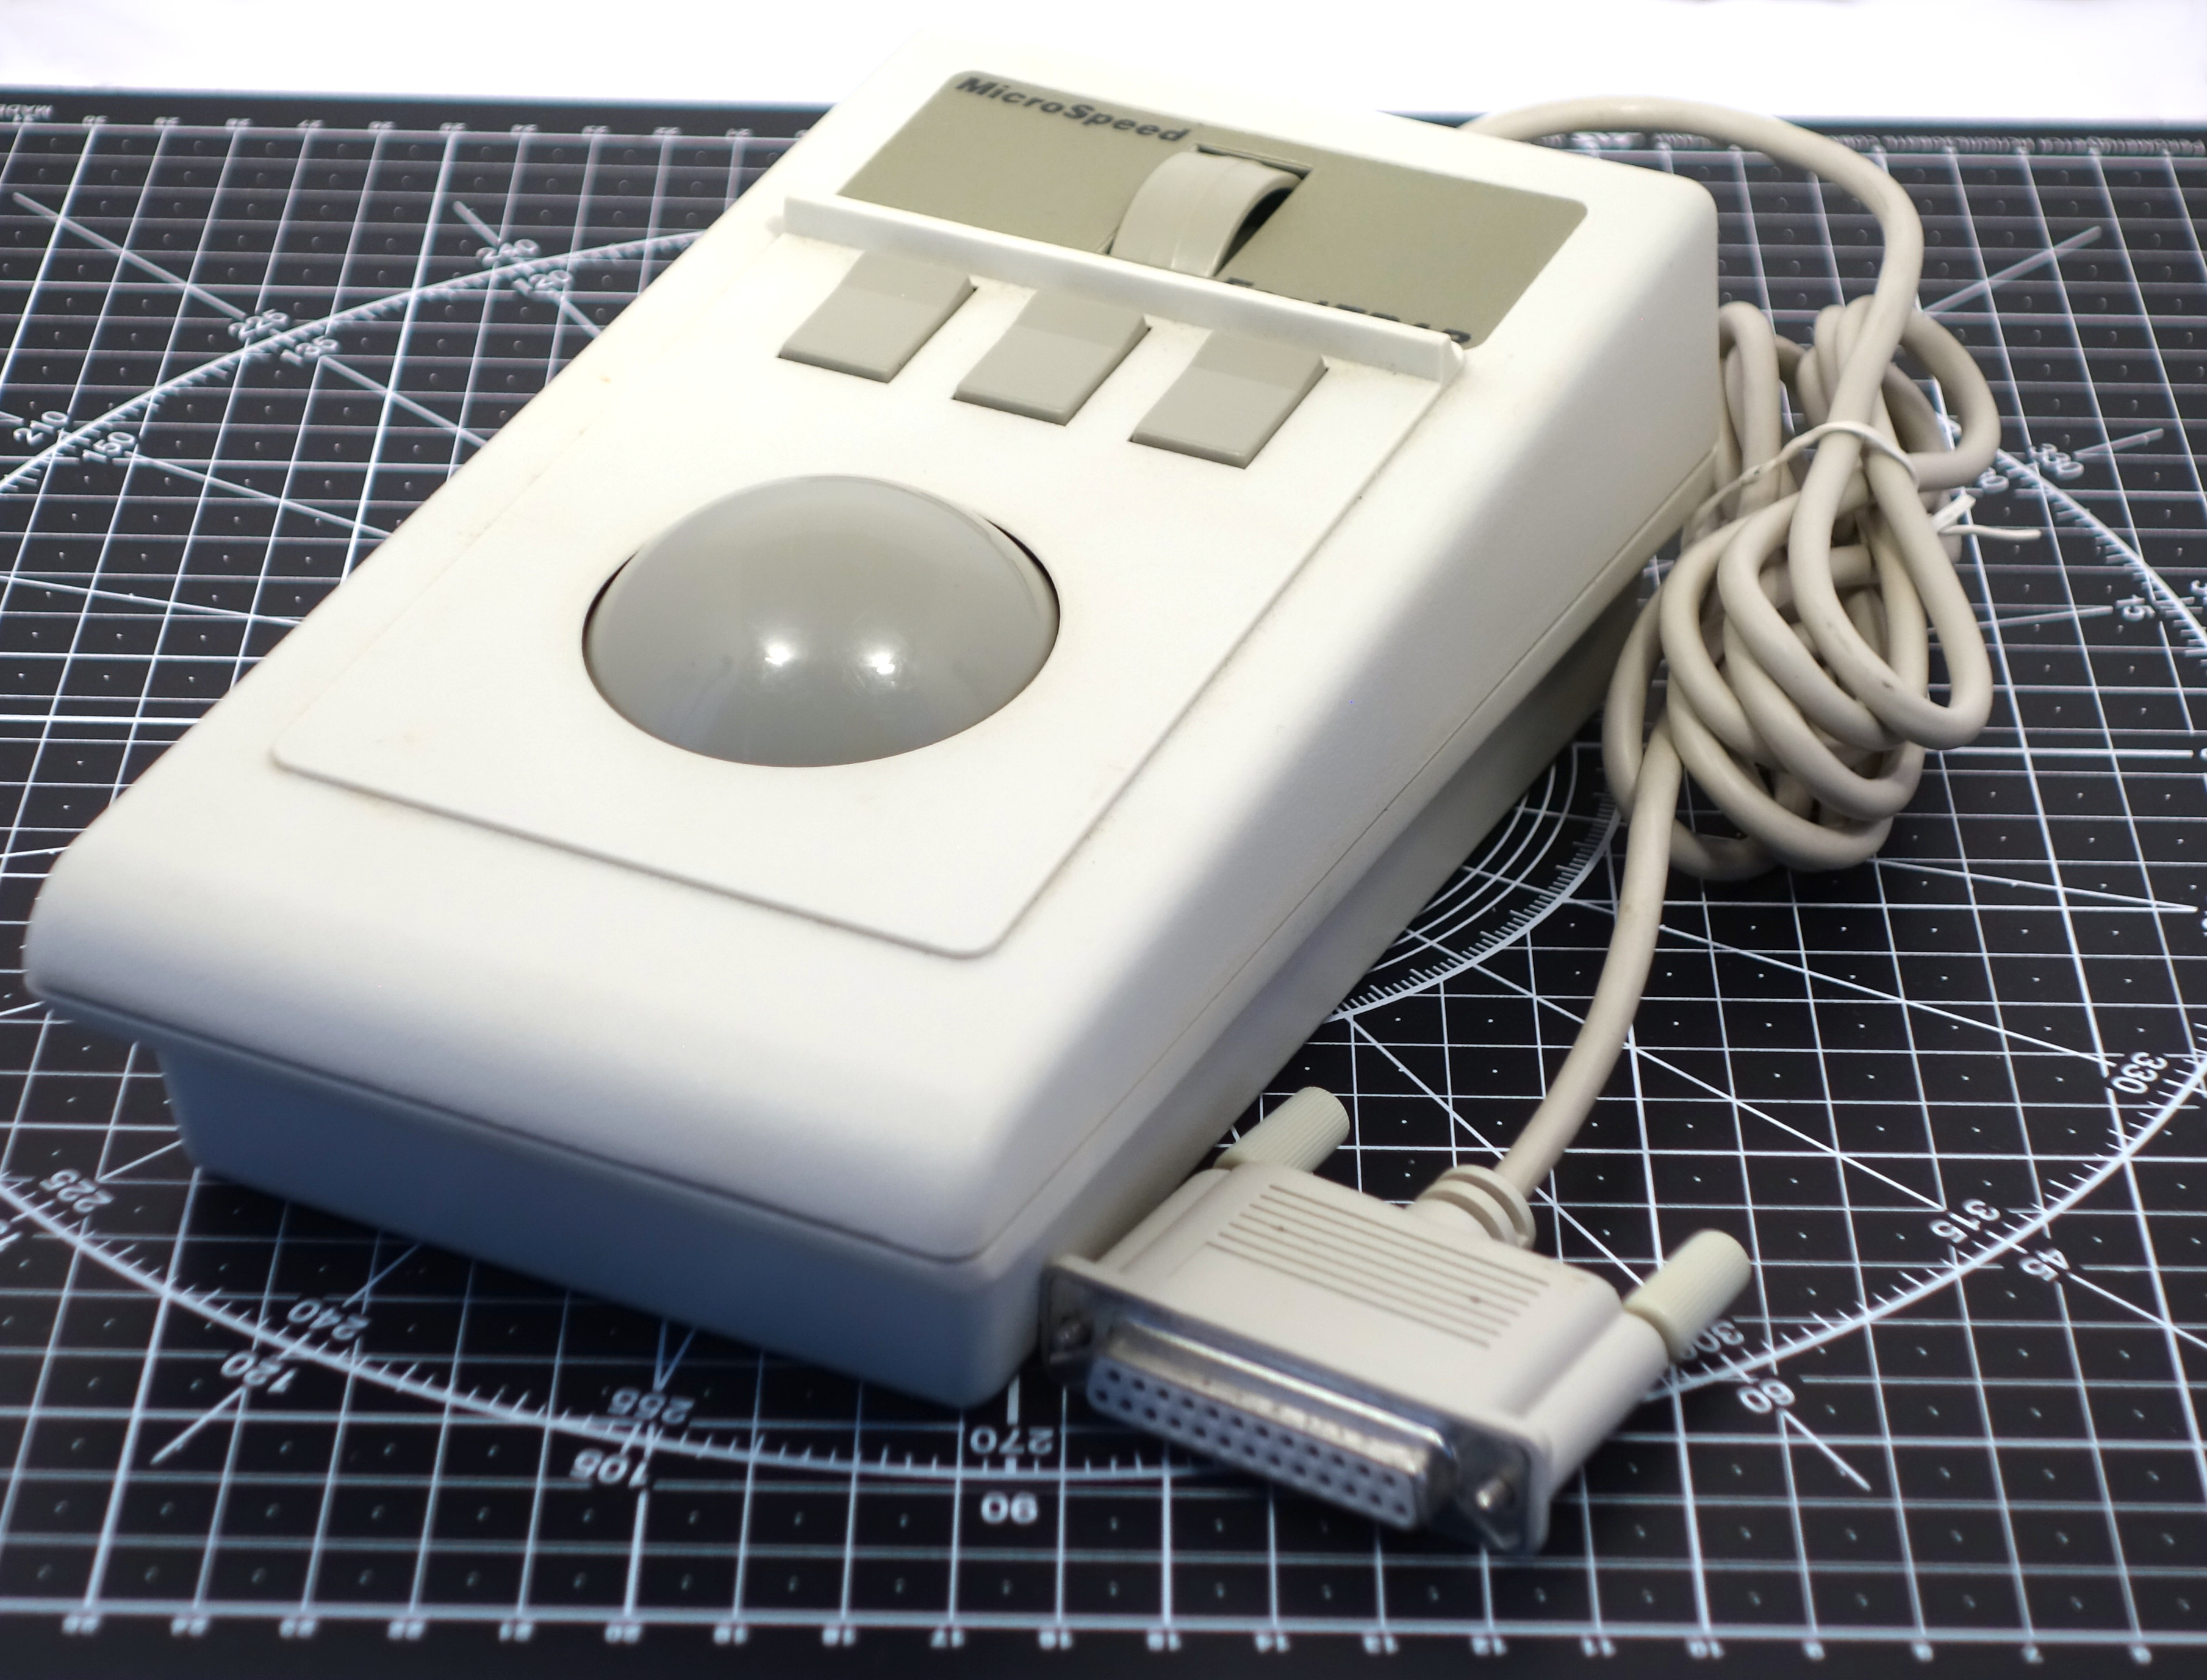
\includegraphics[scale=0.3]{1987_microspeed_fasttrap/size_15.jpg}
    \caption{Изображение FastTRAP на размерном коврике}
    \label{fig:FastTRAPSize}
\end{figure}

Трекбол является очень крупным (рис. \ref{fig:FastTRAPSize}, \ref{fig:FastTRAPHand}). Помимо третьей координаты, FastTRAP предоставляет пользователям САПР дополнительное преимущество за счет большого диаметра шара: точное размещение курсора в графическом окне оказывается точнее проще, чем при перемещении мыши в нужное положение (иногда не удается избежать случайного перемещения мыши при нажатии кнопки).

\begin{figure}[h]
    \centering
    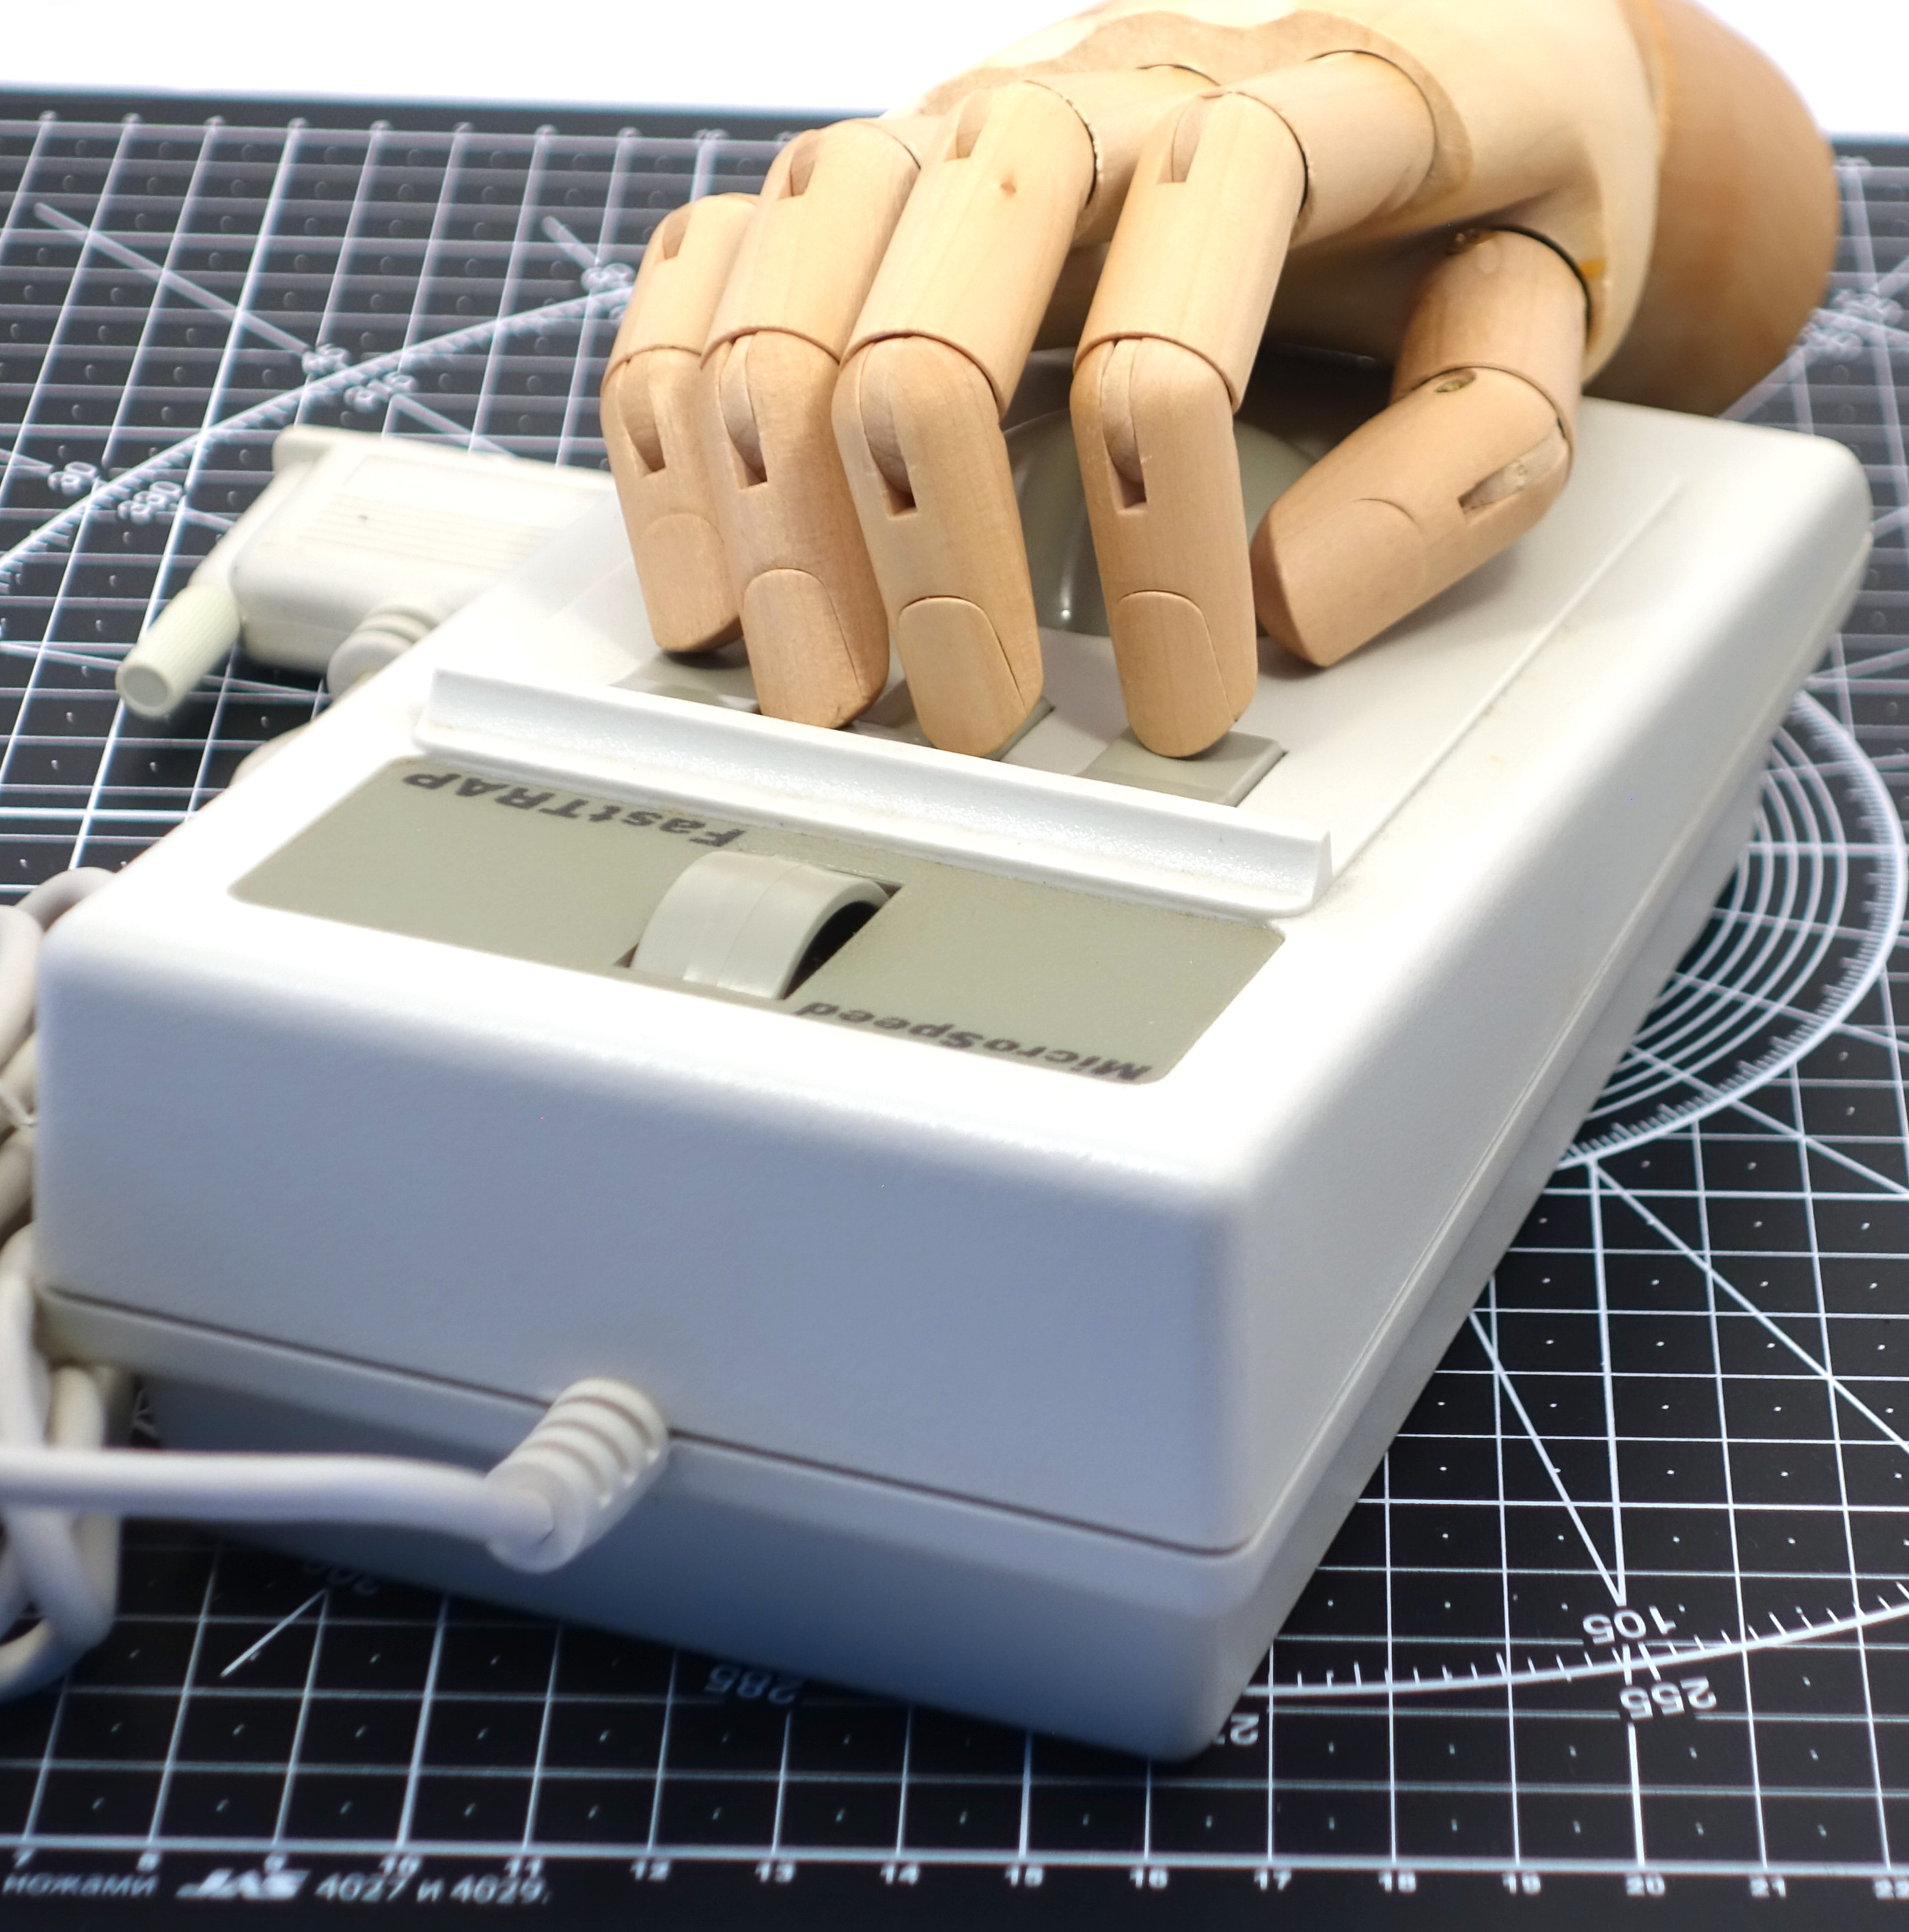
\includegraphics[scale=0.25]{1987_microspeed_fasttrap/hand_15.jpg}
    \caption{Изображение FastTRAP на размерном коврике с моделью руки человека}
    \label{fig:FastTRAPHand}
\end{figure}

В плане эргономики кнопки трекбола расположены достаточно удобно с точки зрения их досягаемости "--- при условии, что пользователь накрывает шар ладонью. Однако колесо находится на дальнем от от пользователя краю корпуса, и для его вращения может понадобиться перемещать руку (рис. {fig:FastTRAPTop}, \ref{fig:FastTRAPHand}).


\begin{figure}[h]
    \centering
    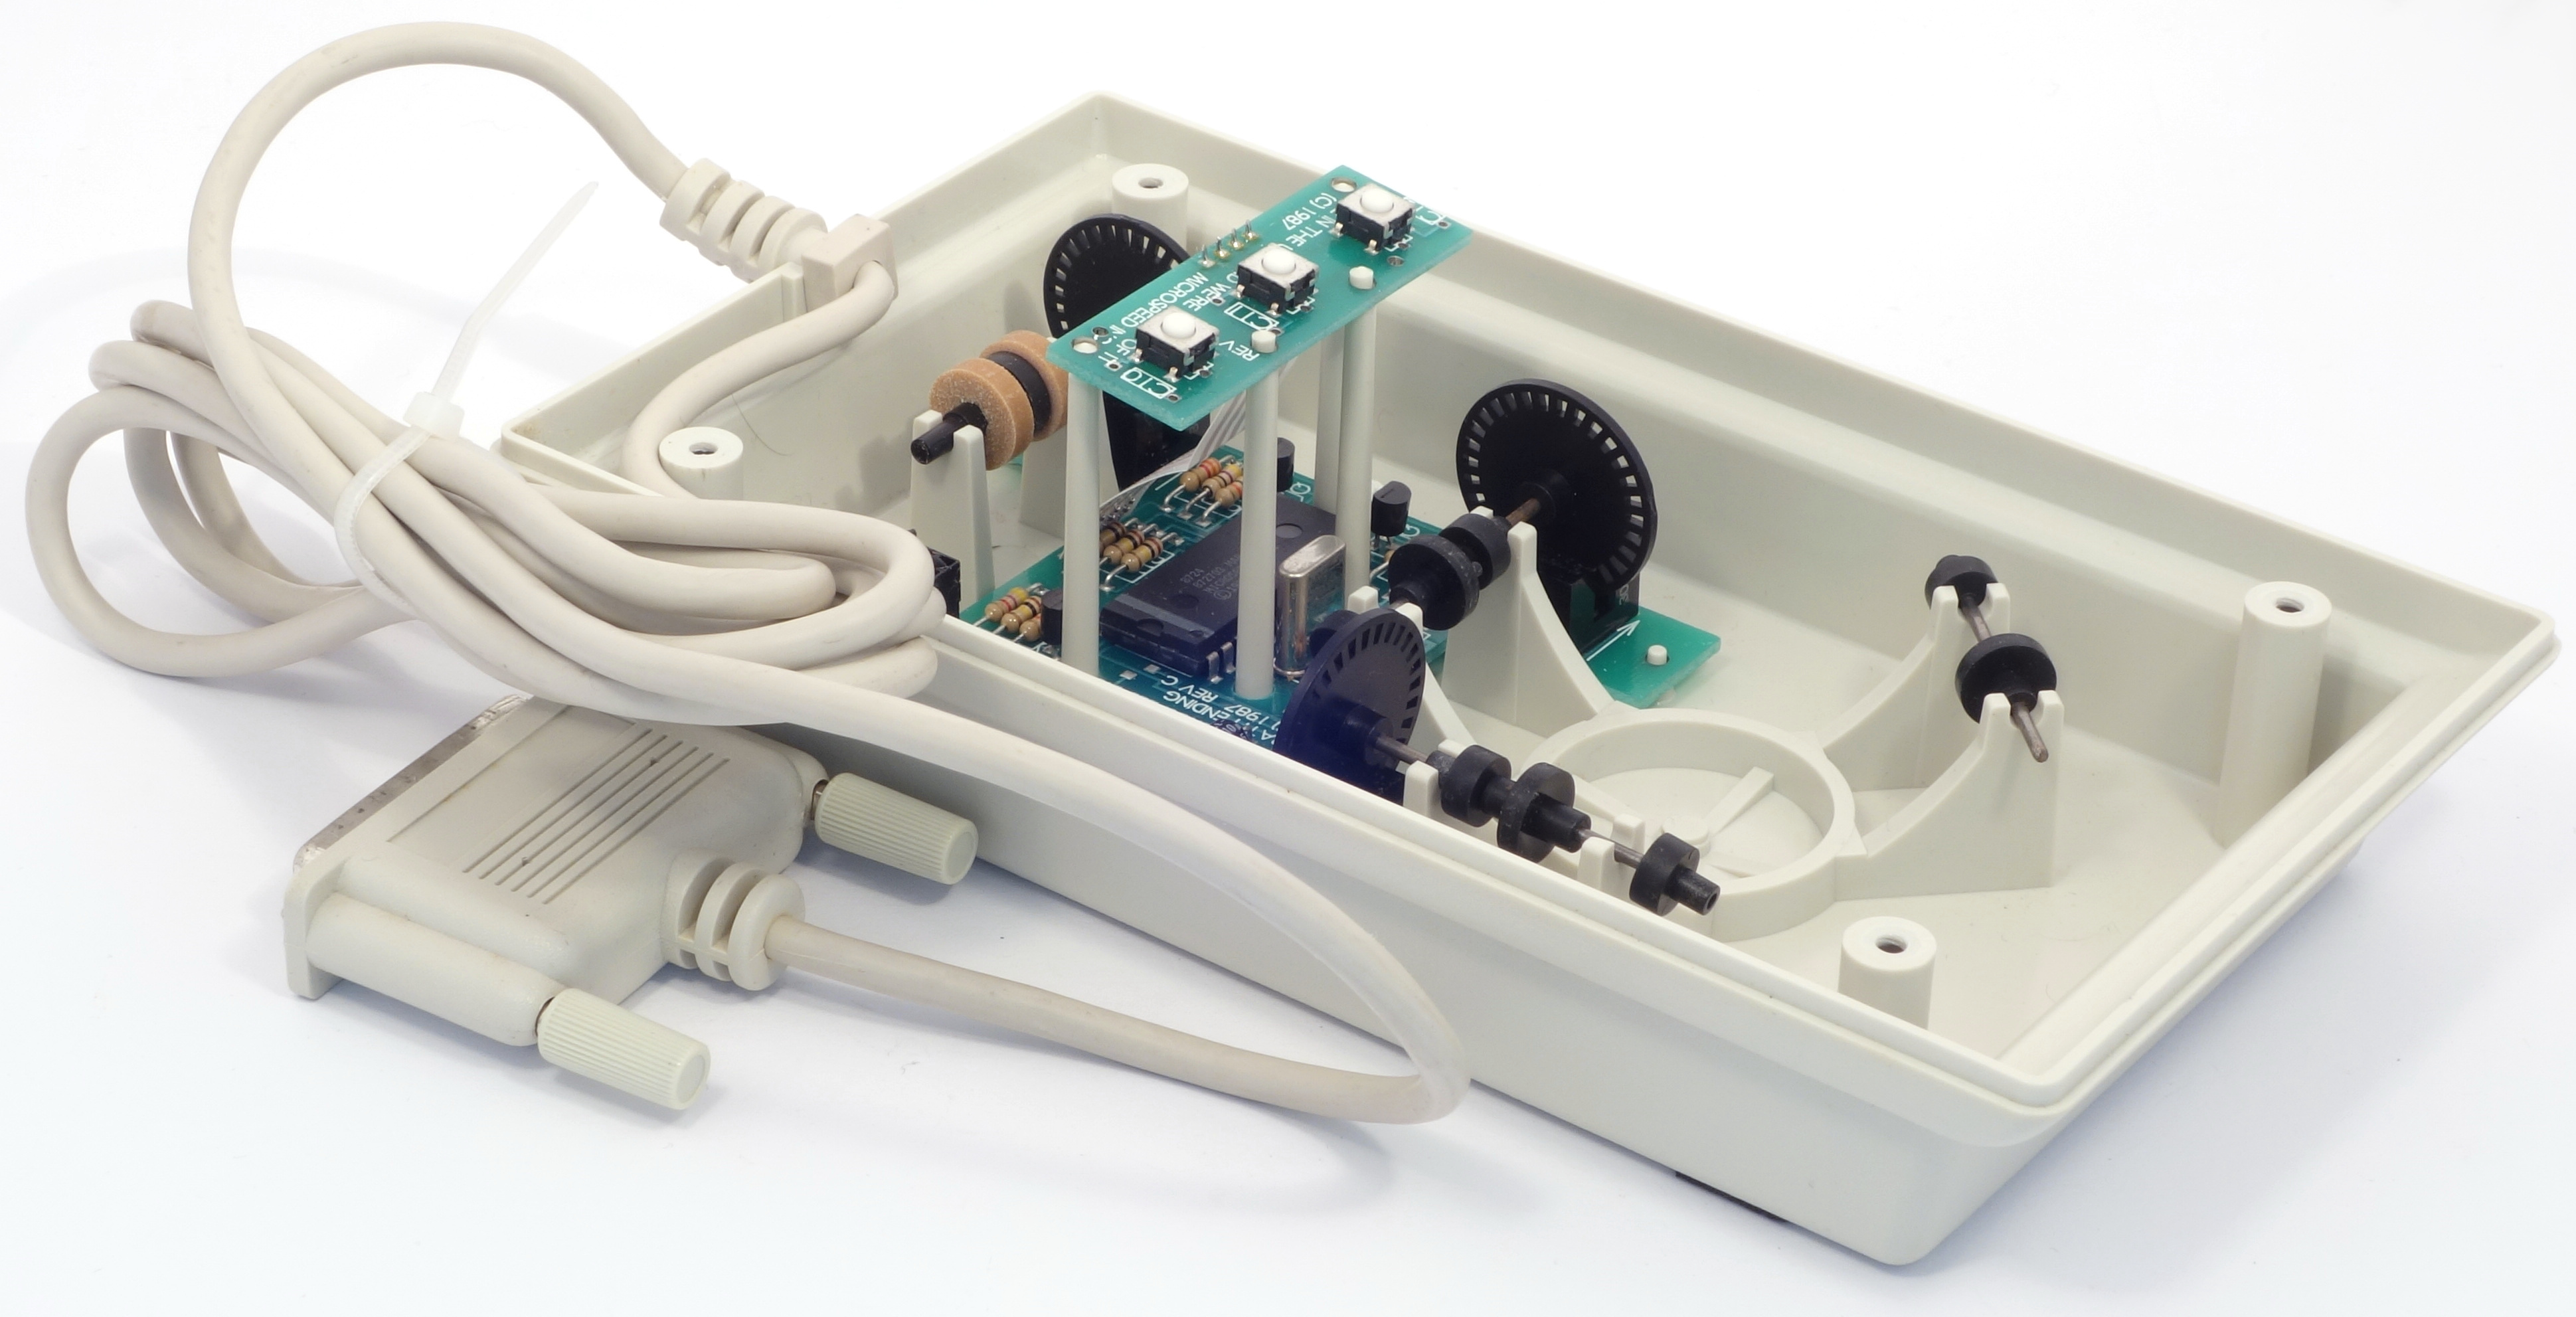
\includegraphics[scale=0.5]{1987_microspeed_fasttrap/inside_15.jpg}
    \caption{Изображение FastTRAP в разобранном виде}
    \label{fig:FastTRAPInside}
\end{figure}

Внутреннее устройство трекбола можно видеть на рис. \ref{fig:FastTRAPInside}.
Стандартная оптомеханическая конструкция дополнена фрикционной передачей, связывающей ролик с дополнительным оптомеханическим энкодером. Также можно заметить идентичность энкодеров, выполняющих снятие перемещения по всем трём осям: с одной стороны, это оказалось не самой сложной задачей в плане компоновки (учитывая большие размеры корпуса), а с другой, это может быть актуальным, учитывая назначение дополнительного колеса.

\begin{thebibliography}{9}
\bibitem {fast} G. Kunkel. The 3-D FastTRAP points with precision // PC Magazine, November 24, 19987. - p. 56.
\end{thebibliography}
\end{document}
